\chapter{Concept and Design}
\label{cha:conceptanddesign}

This section explains the concept and the design of this study. There are three subsections. The first section introduces the concept with general purposes, and the second section presents problems in this study. The last section consists of the overall system structures and compositions of this study.

\section{Concept}

In the distributed P2P network, a peer takes both positions of server and client. Any peer can provide and receive data. Therefore, the P2P network is deployed in diverse areas such as file sharing, media streaming services, distributed websites, and even digital cryptocurrency. Also, any type of device from small IoT to mobile can join the network. Because of its expandability and diverse usability, we consider a distributed network topology, so that IoT devices and PC are able to connect the network and communicate on the distributed DHT network. Example 1 gives an explanation with the considered situation to help with the understanding.

IoT devices in Example 1 are participating in the P2P network as a peer. The network topology consists of XOR-based DHT. Another peer using PC has also joined there. When a PC user wants to upload a new configuration file of more than five megabytes big files, the user stores them on DHT. Conversely, IoT device users should be permitted to download the stored file. Peers retrieve the file through the file name. After the complete lookup, they can successfully download the configuration file. In contrast, the IoT device's peer can push the file, and it is transmittable using the same procedure.

It may be shown as a simple server-client network. However, it is deployed on the distributed overlay P2P network using XOR-based DHT. Moreover, it is the serverless network topology. Therefore, file sharing is readily operating among heterogenous peers through a single application. Furthermore, the peer of IoT devices is able to transmit data to another peer. It means duplex communication should be supported. Data transmission has no limitation on the size of transmittable data and type of data. The system should even have capable implementation in the minimized device such as IoT. In the following section, we describe the system architecture and more details of functionalities.

\section{Problem description}

The problems we have recognized can be divided into two parts. The problems of MTU limitation are explained in the first part. In the second part, the problematic limiting points according to characteristics of IP Protocols are described.

\subsection{MTU limitation}

Ethernet-based network restricts the size of IP MTU (Maximum Transmission Unit). An Ethernet frame normally consists of 18 bytes Ethernet frame overhead and an IP packet. Most networks are universally set to 1500 bytes of the MTU size. Therefore, an Ethernet frame size of 1518 bytes is standardized at IEEE \cite{8457469}. Because there exists a declination of network capacity among physical network properties, data transmission is set to slow, and the allowance of Ethernet frame size is small. Due to this result, this becomes of the obstacles in a modern network system. 

When data transmission is operating between hosts, data will be fragmented into a series of packets. The smaller data is fragmented. The network hop is increasing more. Hence, the network should process fewer packets at the same time. On the contrary, a Network using larger MTU can take higher efficiency because more data can be carried at once. However, larger MTU leads to the increase of network delay in packet processing. Moreover, The packet loss problems causes the network overload to occur.

\subsection{Problematic protocol characteristics}

Before explaining the packet loss problem, it occurs when a network communicates using TCP protocol. If in a TCP communication, where a single bit in a packet is dropped during the data transmission without the FEC scheme, TCP protocol requires the sender to retransmit the entire data. Thus, the payload using a large MTU takes more time in retransmission. When a network exploits a larger MTU, the packet loss rate is increasing \cite{katre2019impact}. The TCP problem involved with MTU is a trade-off between the benefits of large MTU and the risk.

The TCP handshake procedure leads to increased latency. Basically, a TCP handshake has three-phase in connection establishment. Moreover, after the connection establishment, both hosts should establish a crypto handshake. Therefore, the TCP connection establishment requires at least 4 RTT. Peer in P2P networks may frequently connect to new peers in a routing service. We should resolve the presence issue using TCP, which is a connection-oriented protocol.

UDP protocol, which is one of the major internet protocols, is able to be the alternative. UDP may have the advantage in a handshake procedure to TCP because it has no handshake in connection establishment. It needs only a crypto handshake. Therefore, the UDP-based connection needs only 1 RTT in the establishment. The decrease of RTT gives a benefit of latency in the P2P network. If a peer routes several peers, it can reduce the efficiency routing time. However, it is connection-less communication. UDP does not guarantee the reliability of packet loss. When the packet loss occurs between the peers, it is difficult for the peer at the endpoint to detect the packet loss. In multimedia or game communication, it is acceptable, but it can be a critical problem in file sharing. The peer request to send a retransmission of data causes network performance degradation.

Because of the issues that are mentioned above, we consider that this study uses a different protocol or finds efficiency methods for complements to the issues.

\section{Design}

This section explains the composition of applications of this thesis. The section is divided into three subsections. The first section describes the base network system, Staxnet. Afterward, I give an overview of two different scenario applications to resolve the suggesting issues. More detailed implementations and methods will be explained in the following sections.

\subsection{Staxnet}

This section provides an overview of a basic DHT-based P2P network system of Staxnet, which is offered from T-Labs, Telekom Innovation Laboratories. This proto-type system is composed of a DHT daemon application, a command line interface control application, and a certification application. The architecture of Staxnet is illustrated in Figure 3.1. DHT daemon takes networking with parts of other peers. A control application allows the user to access the peer through the daemon and process user commands. Certification application makes the certificates required by the peer establishment.

\begin{figure}[!ht]
	\centering
	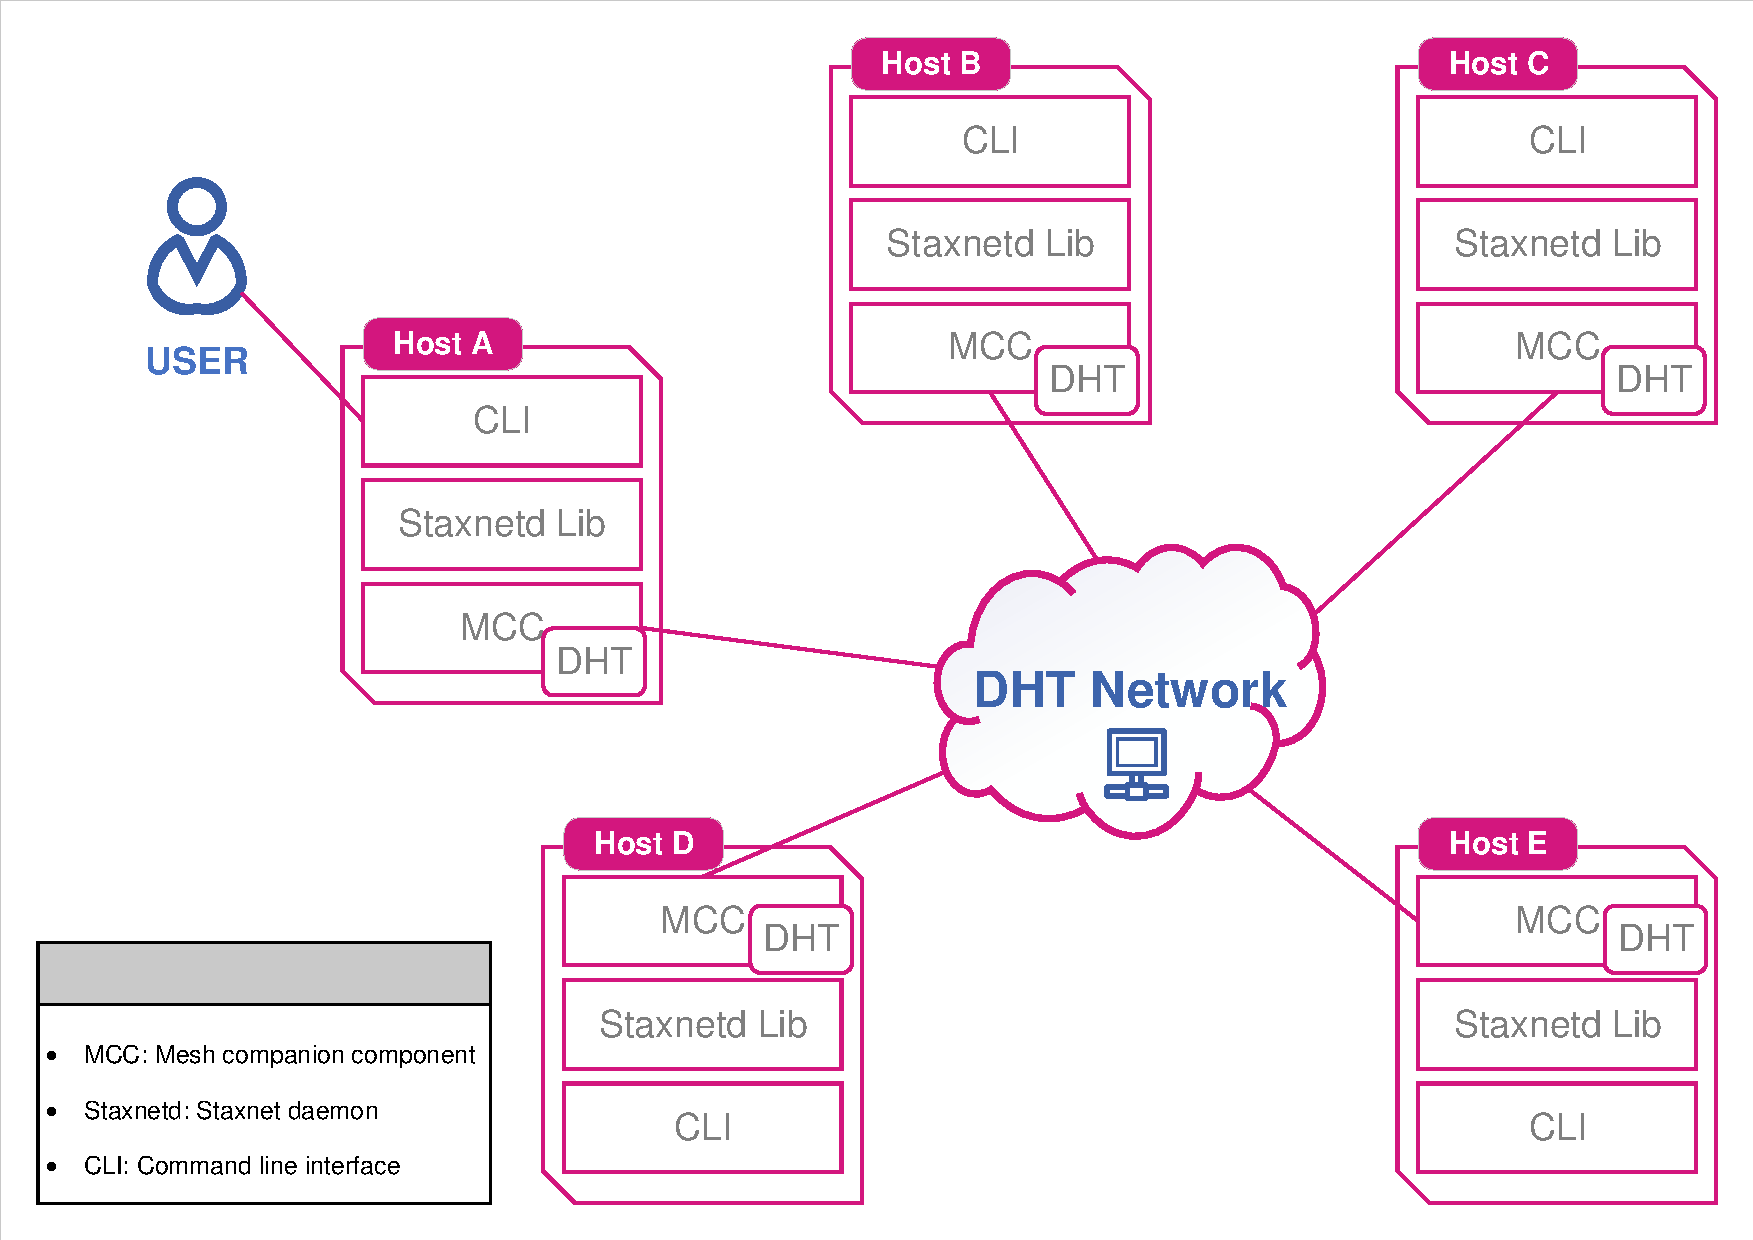
\includegraphics[width=0.5\textwidth]{images/fig_3_1.pdf}\\
	\caption{Overview of Staxnet}
	\label{fig:Staxnet}
\end{figure}

\subsubsection{Staxnet daemon}

Staxnet is designed with mainly DHT daemon and client application. The network is composed of peers, and the peer is controlled by Staxnet daemon application. Peers communicate on this daemon. This application provides following four main functions:

\begin{description}
	\item Peer establishment
	\item Connectivity among peers
	\item DHT Routing table
	\item Certificate handling
	\item Neighbor pinging
\end{description}

Hence, Staxnet daemon application is overall networking management application. Figure 3.2 shows a sequence diagram of the peer creation. 

\begin{figure}[!ht]
	\centering
	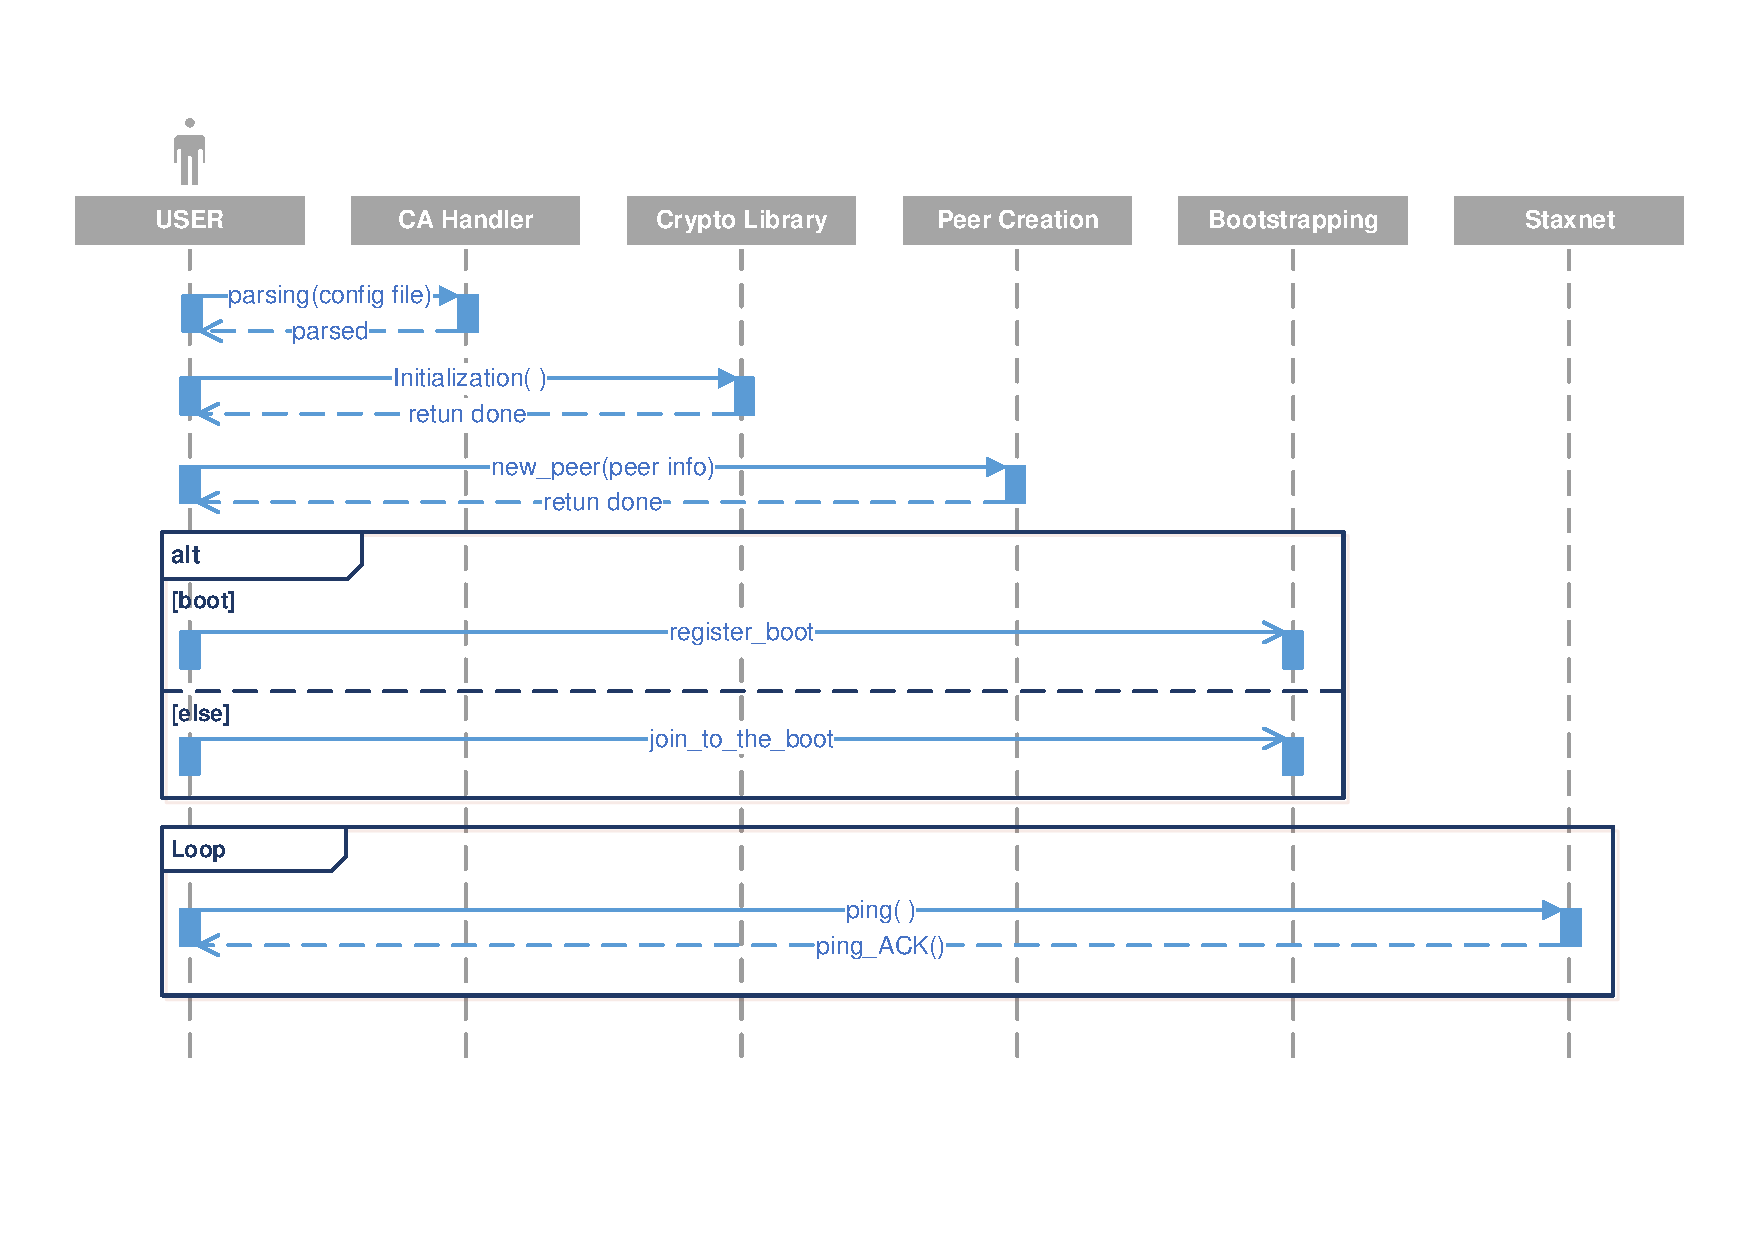
\includegraphics[width=0.5\textwidth]{images/seq3_2.pdf}\\
	\caption{Simplified sequence diagram of Staxnet daemon}
	\label{fig:Staxnet daemon}
\end{figure}

At the beginning of the Staxnet daemon, it must require a configuration file to set a peer; it consists of peer ID, certificate authority (CA), public key, and secret key. A user must ensure the composition of attributes in this given configuration file. If all of the attributes exist, the CA handler extracts information. The daemon initializes the crypto library. All packets, which are used for communication with other peers, will be encrypted by this library, so it needs to be operated before any other function is called. Then, the daemon calls a function with extracted peer information for the creation of a new peer.

In this function, the daemon establishes a memory database. The given key-value will be stored in the DB. Next, a new empty routing table is initialized. After this function, the new node will be initialized at this routing table. Through the given peer information, the daemon verifies certifications. Upon successful completion of all these basic preparation procedures, the process of connecting to the network begins.

The prepared peer in the bootstrapping procedure is established. The daemon regards the first peer as the boot peer. If there is at least one, the next peer is defined as the ordinary peer. The boot peer starts waiting until the other peer attempts to connect to itself. Conversely, the ordinary peer sends a ping message to the boot peer. When the ping returns to it, the connection establishment between peers is exactly completed. After the establishment is completed, the peers keep sending ping messages until peers are disconnected. We explain the initial preparation of the network in this section. The other part, the CLI control application and the lookup service, will be introduced in the following section.

\subsubsection{Command line interface application}

The other part, the CLI application, cannot execute solitary. Therefore, it must connect to the Staxnet daemon. The daemon and CLI application are connected using the Unix socket protocol. It provides functionalities for inputting the key-value and searches the peer. The key-value or key arguments are given from a command line. The provided functionalities are shown in Figure 3.3.

\begin{figure}[!ht]
	\centering
	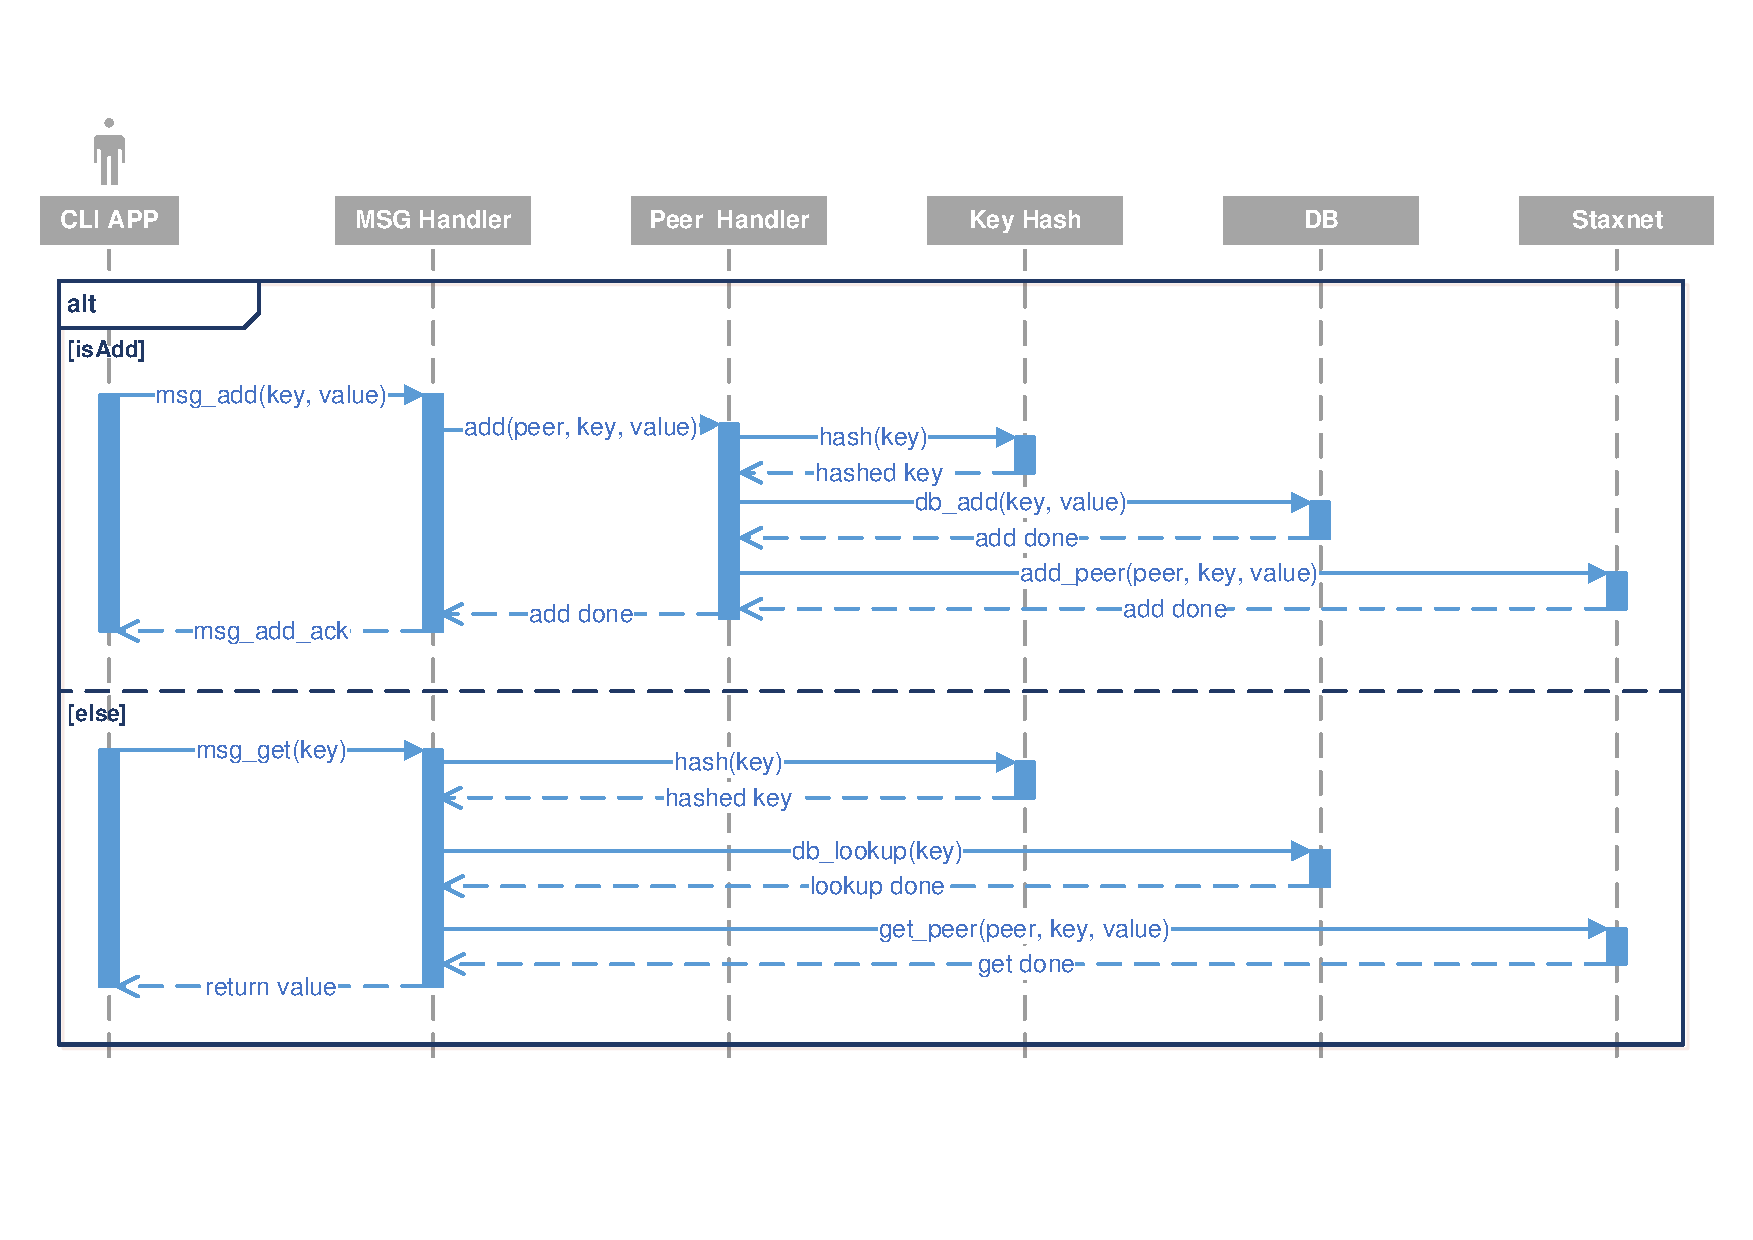
\includegraphics[width=0.5\textwidth]{images/seq3_3.pdf}\\
	\caption{Sequence diagram of CLI application}
	\label{fig:CLI}
\end{figure}

The function is determined by what arguments are received. When the CLI application gets key and value as an argument, a peer is added using the given key-value paired. Otherwise, it searches a value through the given key. The key is a common factor for both functions. In the add function, the CLI application gets sent to the Stax daemon the RPC message, \textit{msg\_add( )}, with a given key and value. The message handler in the daemon begins a procedure of adding key and value and calls a peer handler. At this procedure, the peer handler initializes for the given key and value. It allocates space for store data. The given key gets sent to the hash function. The key is hashed there, and then it will be returned. The received key-value paired is added using the hashed key in the DB. The initialization of peer is hereby completed. The daemon gets a peer list of the bucket from the routing table. The data will transverse the bucket on the Staxnet network according to the DHT protocol.

On the other hand, the CLI application gets only a key argument. The application sends the daemon to the different RPC message, \textit{msg\_get( )}, including the given key. The daemon hashes the given key, and then it starts a lookup service of its own DB; if the matched data does not exist in the DB, the peer is set as an empty DB. The daemon transmits to the routing table with the peer, including searched DB and the given key-value paired. The routing table offers a list of the bucket. The daemon sends to peers in the list the request. If the matched data are found from any peer, the daemon compares both data. At last, the selected data will be returned to the CLI application.

Above we explain the design of CLI application. The following section describes the routing table.

\subsubsection{Routing table}

The Staxnet daemon exploits XOR-based Kdemlia DHT. The detail of the description is explained in Section 2.4. When the daemon executes lookup or add a new peer, the routing table must provide the list of the bucket. Figure 3.4 shows the simplified routing table.

\begin{figure}[!ht]
	\centering
	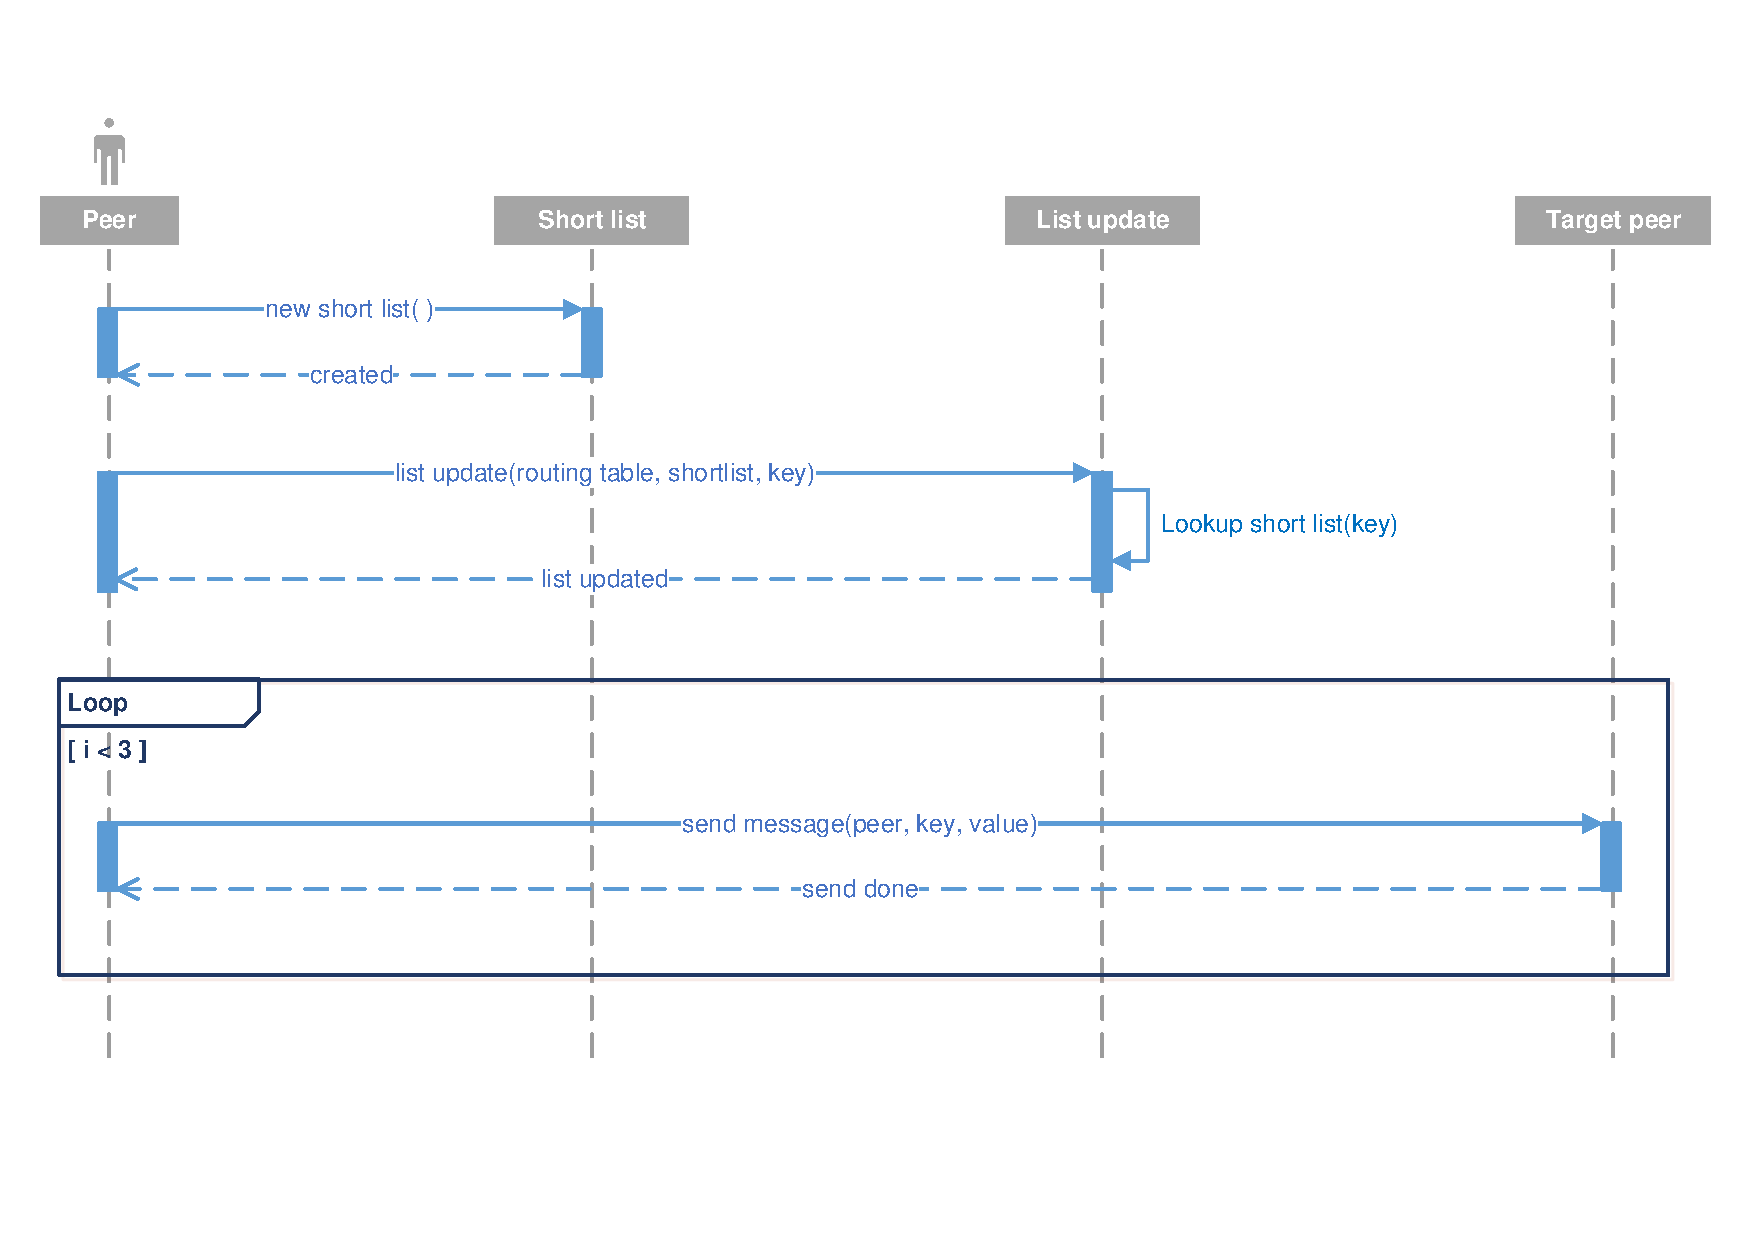
\includegraphics[width=0.5\textwidth]{images/seq3_4.pdf}\\
	\caption{Sequence diagram of routing table}
	\label{fig:routing table}
\end{figure}

At first, a peer should allocate the empty shortlist, which is the short distance peers in a bucket. The routing table looks up an existing shortlist. The routing table calculates a distance between the peer and the given key. If the shortlist is empty, it starts making a new shortlist. Otherwise, it compares the distance between the calculated distance and the distance in the shortlist. After the shortlist update, the routing table propagates to the three near peers of the updated shortlist. Using this procedure, DHT always updates its bucket and provides efficient features of Kademlia DHT.

We consider two models, all peers propagation model and direct tunnel-based P2P model, to compare efficient data transmission. In the following sections, we explain the design of each plan.

\subsection{All peers propagation model}

All peers propagation model is the basic Kademlia DHT-based data transmission model. It is based on providing the Staxnet daemon and the CLI application. However, the legacy system gets the key and small value that restricts the size of the payload until 1500 bytes. The limited size of the payload is according to MTU size. When a user sends a large file such as media contents, the size of the file will be up to 1500 bytes. Therefore, this model sets the key and value list paired instead of the legacy key-value paired. In the memory DB of the system, the key is the head of a linked list, and the value will be stored in the lists. We consider how to utilize the existing given system as much as possible without modification. Therefore, the DB tries to use the existing memory DB without installing a new external DB. In addition, the data transmission method between peers proceeds in the same manner as in the existing system architecture. Figure 3.5 is described to help to understand the overview of the all peers propagation model.

\begin{figure}[!ht]
	\centering
	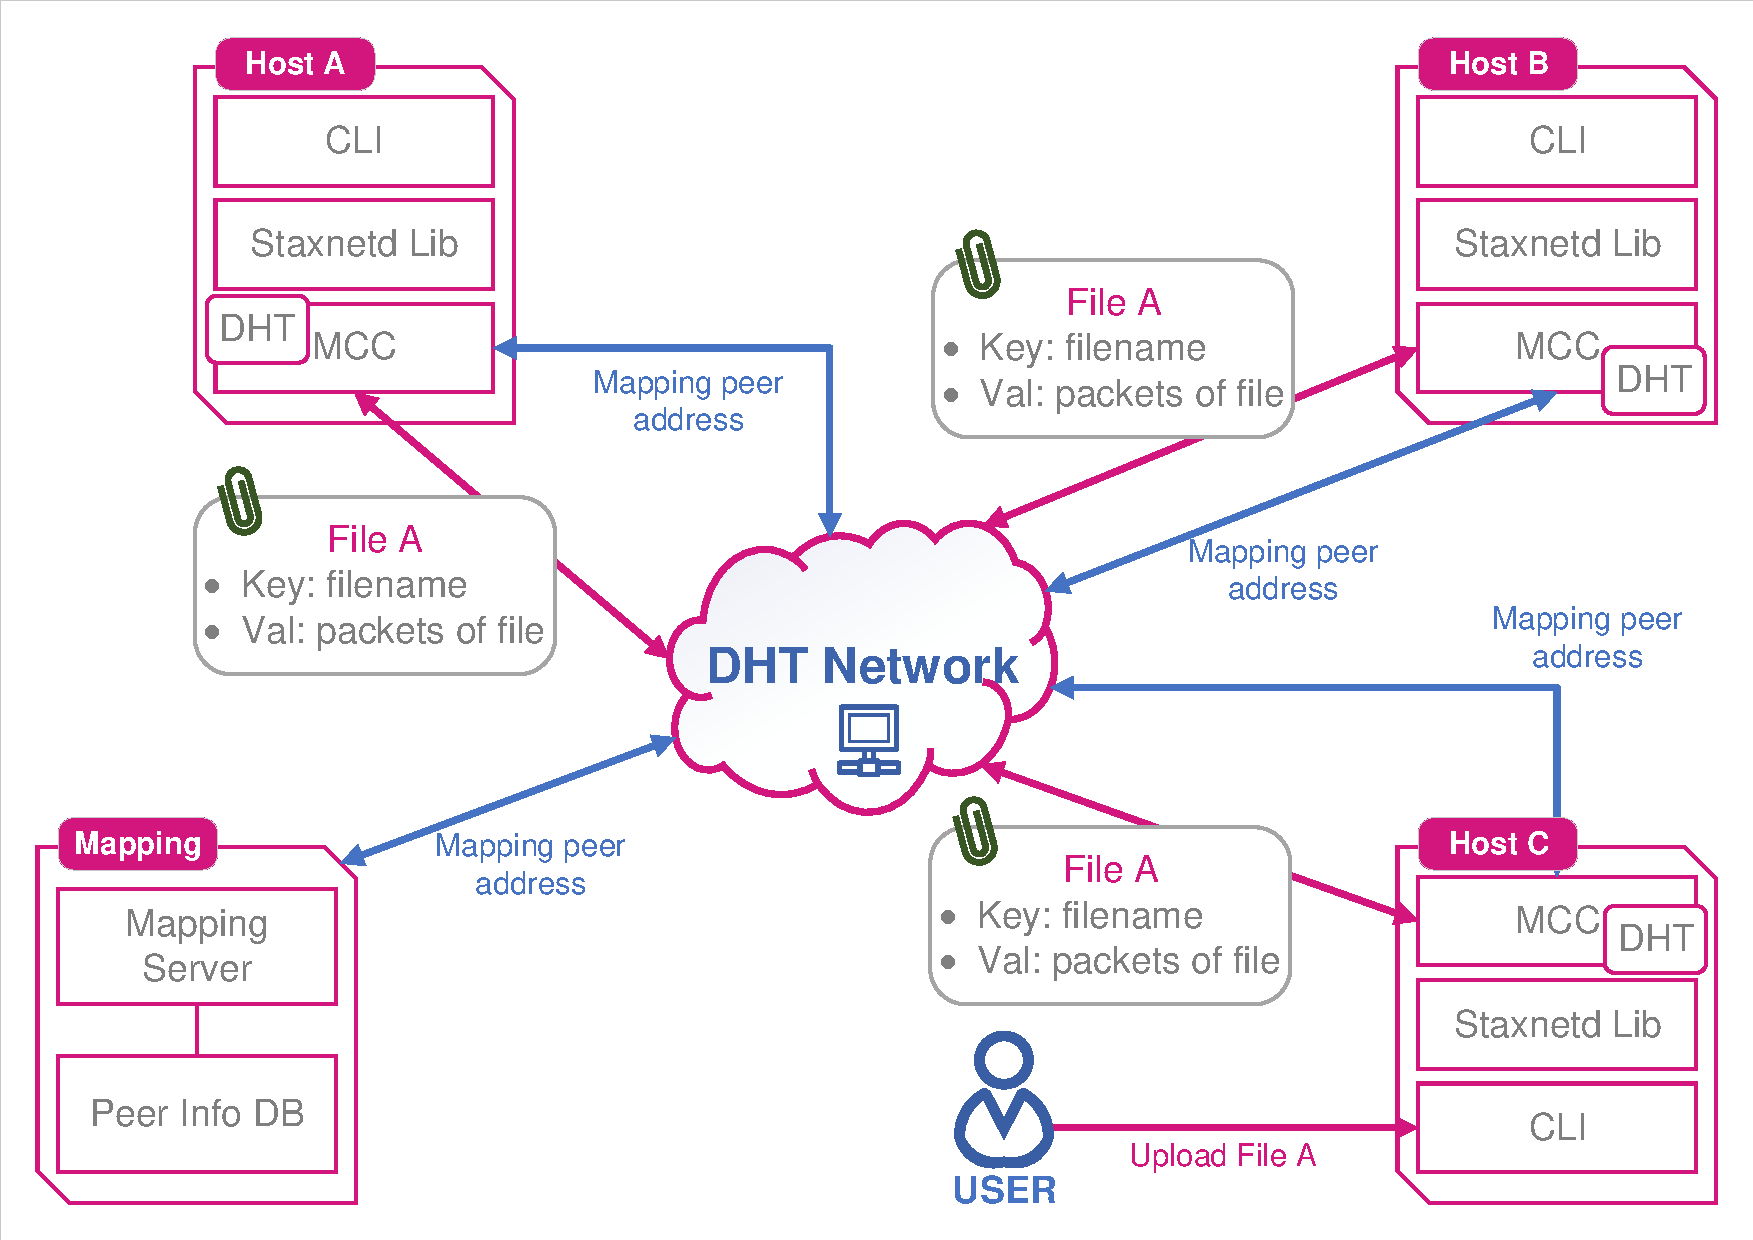
\includegraphics[width=0.5\textwidth]{images/fig_3_5.pdf}\\
	\caption{Use case of all peers propagation mode}
	\label{fig:all peers}
\end{figure}

This model has a mapping server. The existing system's configuration file includes the IP address of the boot peer because Staxnet requires a bootstrapping peer to configure the network. The mapping server utilizes to avoid exposure of the address in the external file. Whenever a peer establishes at Staxnet, it executes its address on the mapping server. Other key-value paired transfer methods are the same as those described above.

\subsection{Direct tunnel-based Peer-to-Peer model}

In the all peers propagation model, the upload data must process at least two times to read the whole data. If the size of the file is not big, it is able to read quickly. Otherwise, it must consume much time, and it causes performance degradation. That is why we consider with a different method. The uploading file will be read on the command line interface, and the peer stores only a key that has the file name, and a value that has a peer ID. This paired key-value occupies a small size of data. Therefore, it can give an advantage of reducing the processing time. Figure 3.6 shows the use case of the direct tunnel-based P2P model.

\begin{figure}[!ht]
	\centering
	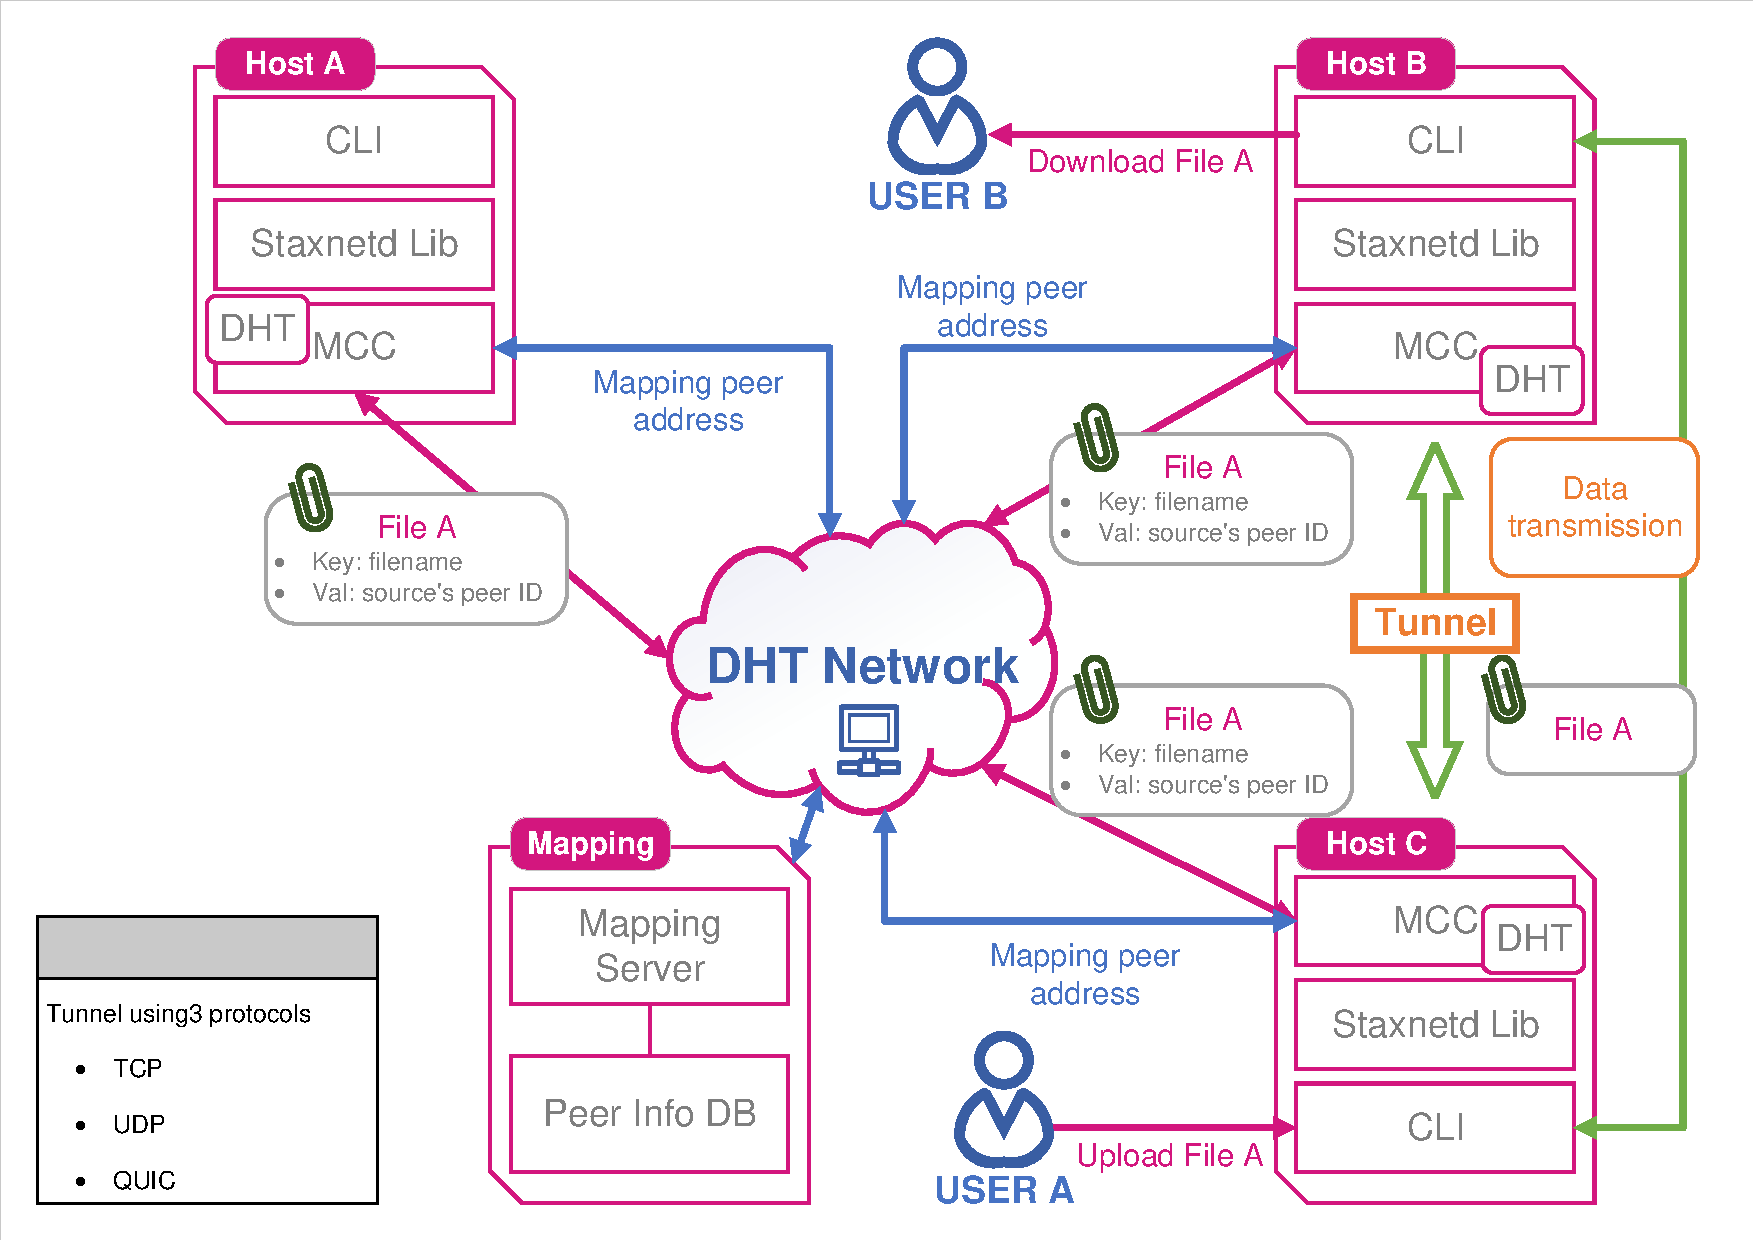
\includegraphics[width=0.5\textwidth]{images/fig_3_6.pdf}\\
	\caption{Use case of the direct tunnel based P2P model}
	\label{fig:tunnel}
\end{figure}

When user A uploads file A, Stax daemon registers a key-value of file A in DHT and transmits it to peers in a bucket. The CLI application is ready to send a file and waits for a download request from another peer. As user B wants to download file A, user B sends a request message with the filename from the CLI application to its Staxnet daemon. It starts the retrieval of file A. When it succeeds, the Staxnet daemon returns to the CLI application, being the retrieved key-value paired data. The CLI application sends another message to the mapping server to get the target’s IP address and port number using the given target’s peer ID. The mapping server responds to the information, and then user B’s CLI application tries to connect to user A’s CLI application. After the connection is successfully established, a direct tunnel is made between both users. The requested data are transmitted via the tunnel. We are confident that this method will improve transmission performance because P2P communication is established through a single tunnel directly connected between the two peers. We have selected a choice of three communication protocols for experimental comparison. When the user configures the upload or download of a file, the user must select a communication protocol in advance. We provide TCP, UDP, and QUIC protocols.